\chapter{Methoden}

\section{Vorgehensmodell}

Als Projektmethode wurde das hybride Modell SoDa festgelegt. Dieses besteht aus den drei Phasen \textit{Initialisierung}, \textit{Konzeption / Realisierung} und \textit{Einführung}. Da die  \textit{Konzeption / Realisierung} Phase inkrementell ist, kann man einfacher auf neue Anforderungen oder Änderungen am Umfeld reagieren. (\cite{sodawebpage})

\subsection{Projektstrukturplan}
\label{ch:Projektstrukturplan}
Der Projektstrukturplan gibt eine Übersicht über die Projektabschnitte Initialisierung, Konzeption/ Realisierung sowie Einführung. Weiter sind die wichtigsten Teilaufgaben zu jedem Projektabschnitt aufgeführt.
\begin{figure}[htb]
	\centering
	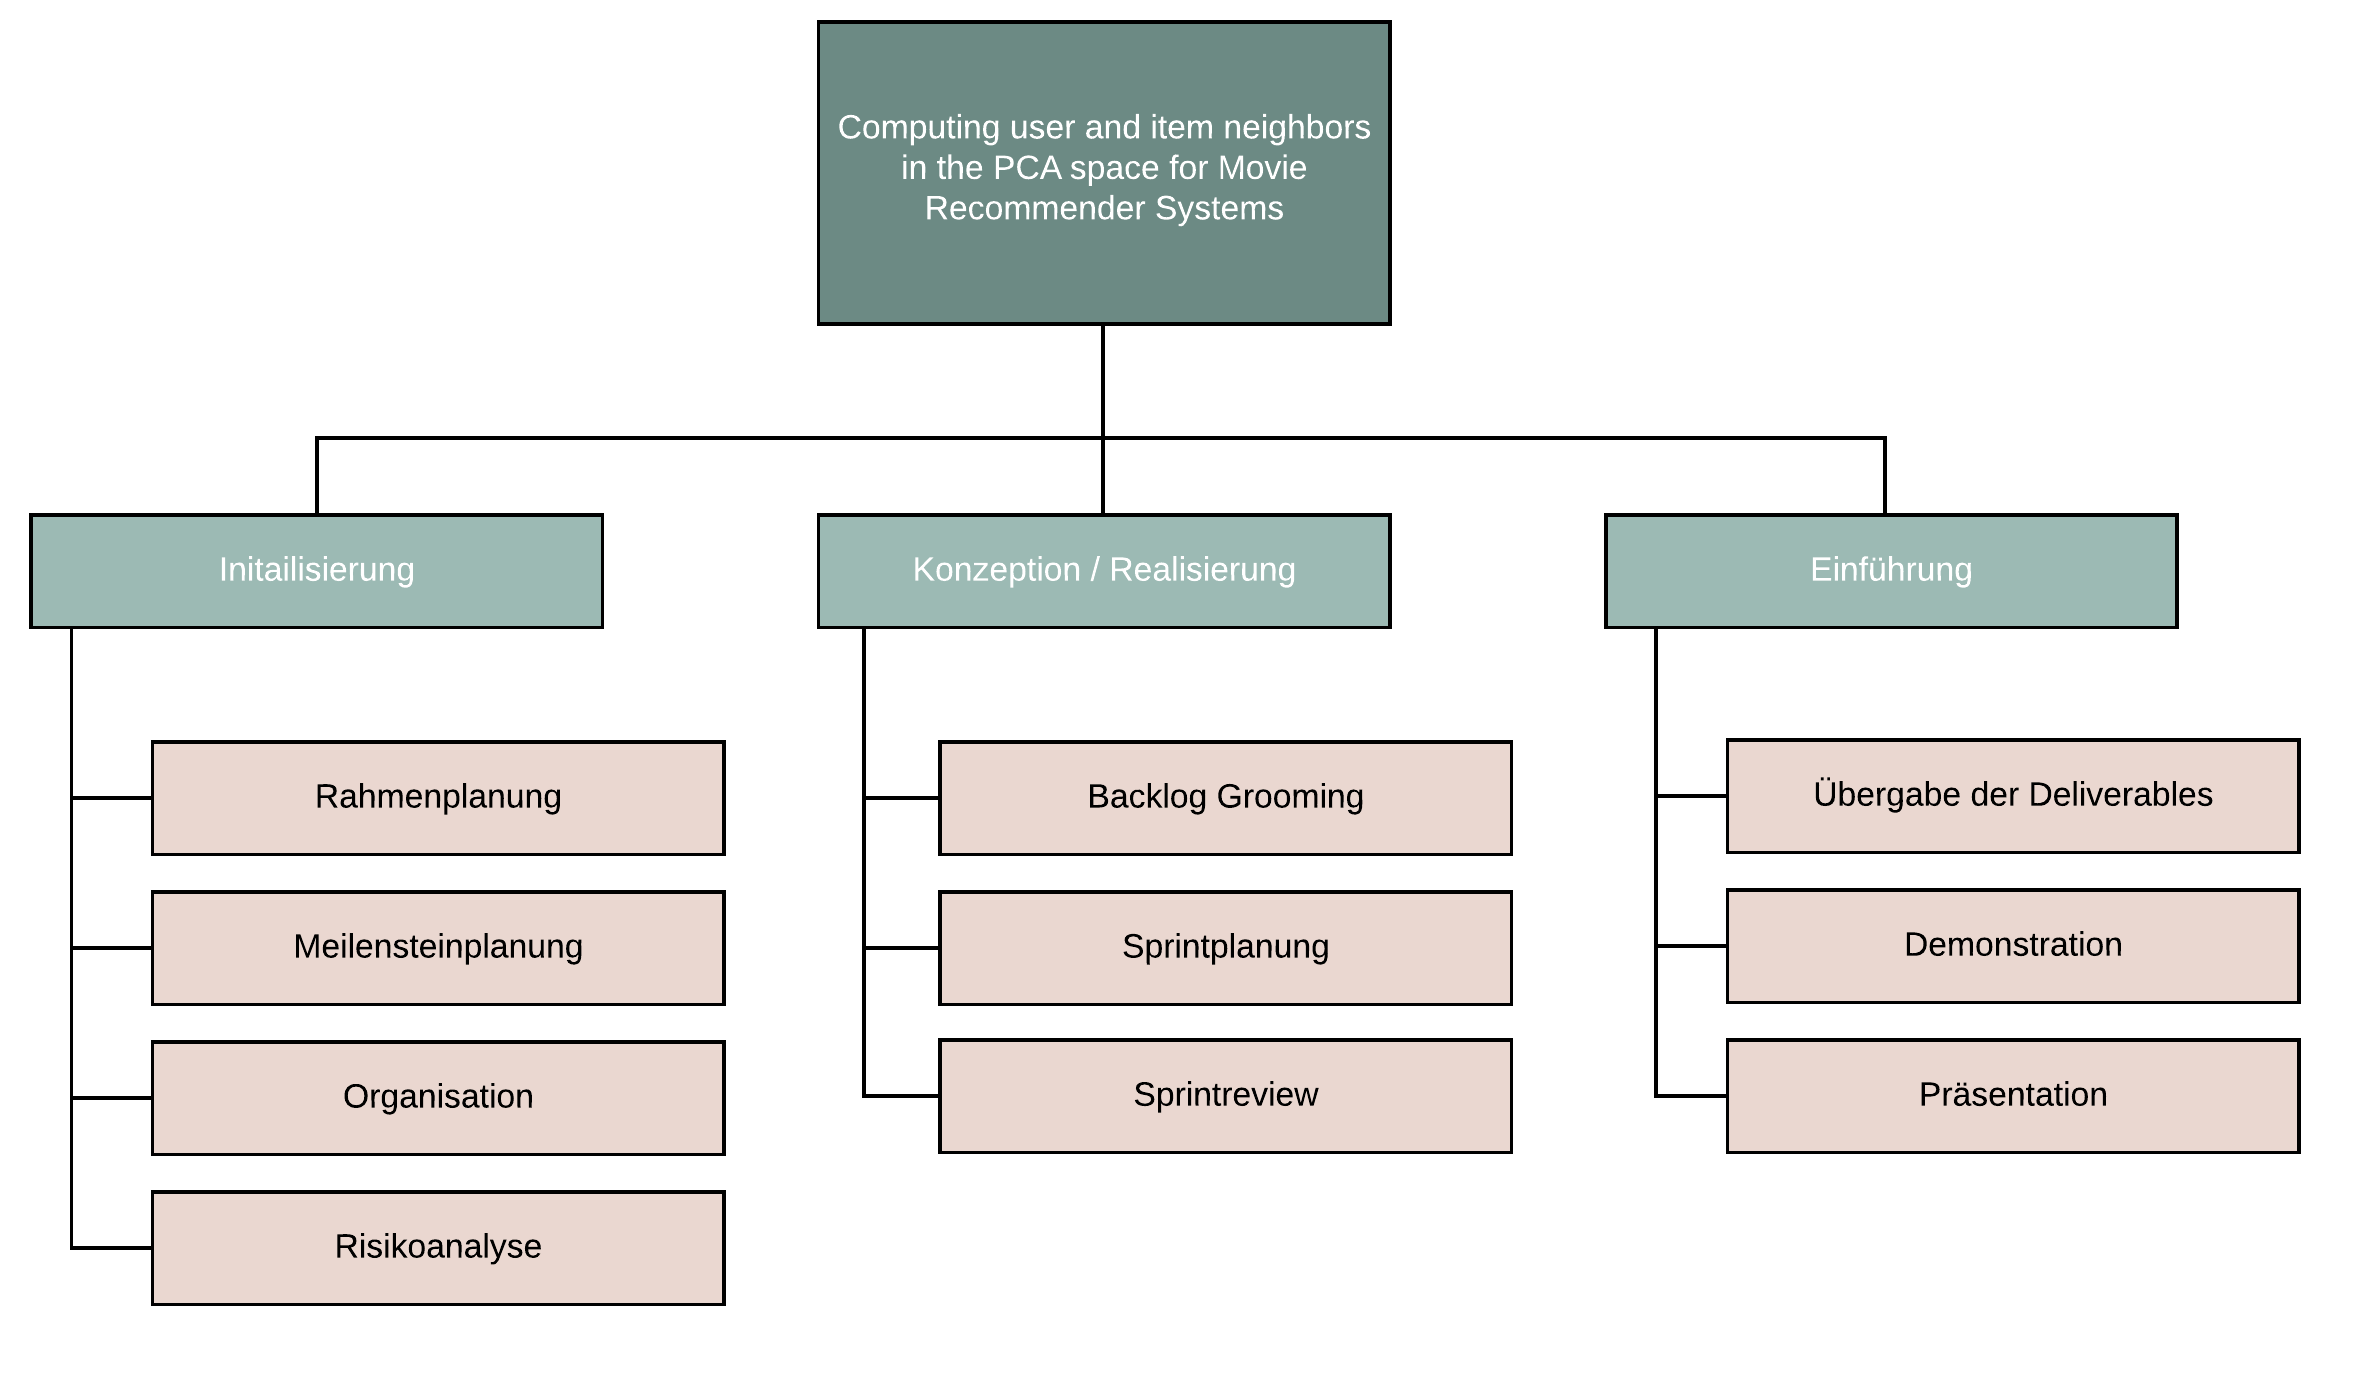
\includegraphics[keepaspectratio,width=\linewidth]{img/Projektstrukturplan.png}
	\caption{Projektstrukturplan}
	\label{fig:Projektstrukturplan}
\end{figure}


\section{Projektführung}

\subsection{Rahmenplan}
Der Rahmenplan visualisiert die Übersicht über die Meilensteine, Sprints sowie den allgemeinen Verlauf des Projekts. Für das Projekt \textit{Computing user and item neighbors in the PCA space for Movie Recommender Systems} wurde der Rahmenplan grösstenteils durch den Projektauftrag festgelegt.

\begin{figure}[htb]
	\centering
	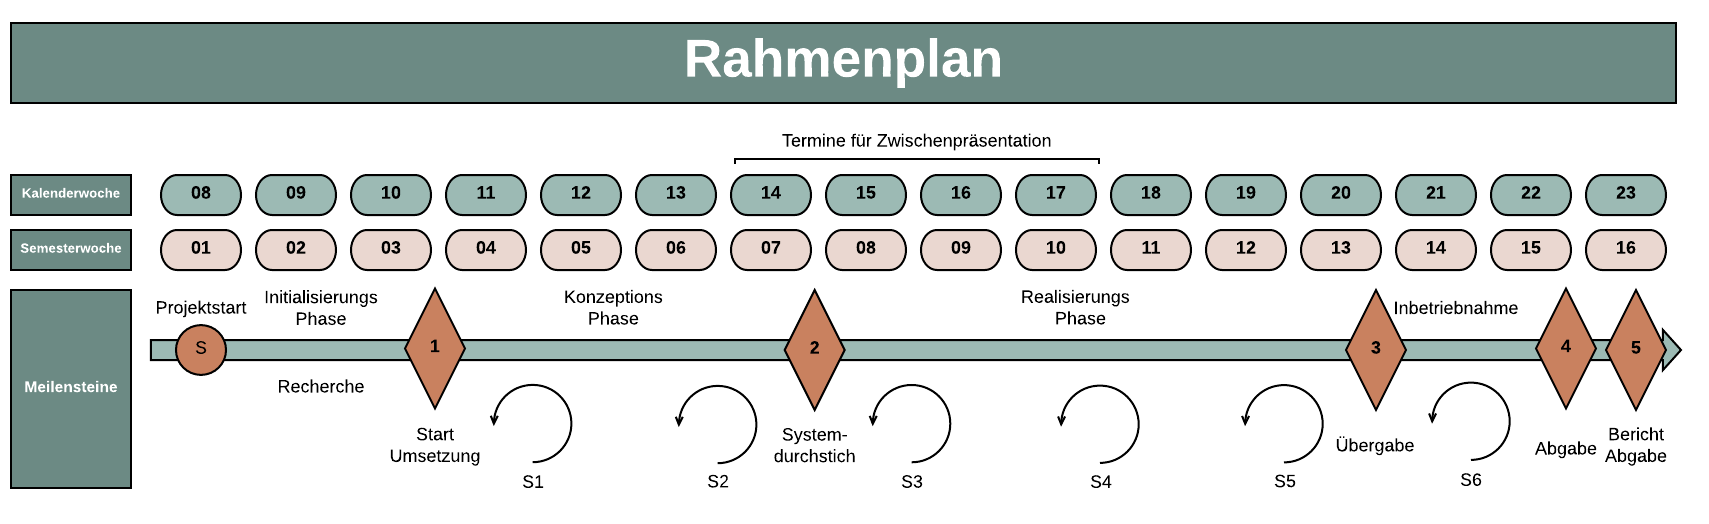
\includegraphics[keepaspectratio,width=\linewidth]{img/Rahmenplan BA.png}
	\caption{Rahmenplan}
	\label{fig:Rahmenplan}
\end{figure}

\subsection{Meilensteinplan}
\subsubsection{Meilenstein 1 - Start der Umsetzung}
Der Meilenstein 1 gilt als abgeschlossen, wenn folgende Punkte erreicht sind:
\begin{itemize}
  \item Initiale Risikoanalyse gemacht
  \item Productbacklog Einträge anhand der Aufgabenstellung erstellt
  \item Erste Version des Grobkonzepts erstellt
  \item Recherche abgeschlossen
  \item Sprintplanung des ersten Sprints abgeschlossen
  \item Rahmenplan erstellt
\end{itemize} 

\noindent Lieferbare Objekte:\hfill Datum: 08.03.2020


\begin{itemize}
  \item Grobkonzept in erster Version
  \item Anforderungen im Productbacklog
  \item Initiale Risikoanalyse
  \item Sprintplanung von Sprint 1
  
\end{itemize}

\subsubsection{Meilenstein 2 - Systemdurchstich}
Der Meilenstein 2 gilt als abgeschlossen, wenn die ersten Grundfunktionalitäten exemplarisch als Prototyp entwickelt und getestet wurden.\newline
\newline
Lieferbare Objekte:\hfill Datum: 05.04.2020


\begin{itemize}
  \item Sprintreview von Sprints 1 und 2
  \item Sprintplanung für Sprint 3
  
\end{itemize}

\subsubsection{Meilenstein 3 - Übergabe}
Der Meilenstein 3 gilt als abgeschlossen, wenn die Software erfolgreich dem Auftraggeber übergeben wurde.\newline \newline
Lieferbare Objekte:\hfill Datum: 17.05.2020


\begin{itemize}
  \item Sprintreview von Sprints 3, 4 und 5 
  \item Auftraggeber hat Zugriff zum Git Repo
  
\end{itemize}

\subsubsection{Meilenstein 4 - Abgabe}
Der Meilenstein 4 gilt als abgeschlossen, wenn die die Software stabil läuft. Ausserdem müssen alle Fehler welche bei der Übergabe aufgetaucht sind, behoben sein.\newline \newline
Lieferbare Objekte:\hfill Datum: 17.05.2020


\begin{itemize}
  \item Stabil Funktionierende Software
\end{itemize}

\subsubsection{Meilenstein 5 - Schlussabgabe}
Der Meilenstein 5 gilt als abgeschlossen, wenn der Bericht erfolgreich eingereicht wurde.\newline \newline
Lieferbare Objekte:\hfill Datum: 05.06.2020

\begin{itemize}
  \item Bericht als PDF/A Dokument
\end{itemize}

\subsection{Sprintplan}
Die Konzeptions-, Realisierungs- und Inbetriebnahme-Phase des Projektes ist in 6 Sprints aufgeteilt. Die Dauer eines
Sprints wurde auf 2 Wochen festgelegt. Die Start- und Endtermine, sowie die Sprintziele sind in folgender Auflistung ersichtlich: \newline \newline

\begin{table}[htb]
    \caption{Sprintplan}
    \label{Sprintplan}
    \begin{tabularx}{\textwidth}{|l|l|l|X|}
    	\hline 
    	\textbf{Sprint} & \textbf{Dauer} & \textbf{Phase} & \textbf{Artefakte} \\
    	\hline 
    	Sprint 1 & 09.03.2020 - 22.03.2020 & Konzeption/ \newline Prototyping & Sprintreview Sprint 1 \newline Sprintplanung Sprint 2 \newline aktualisierter Backlog\\ 
    	\hline 
    	Sprint 2 & 23.03.2020 - 05.04.2020 & Konzeption /\newline Prototyping & Sprintreview Sprint 2 \newline Sprintplanung Sprint 3 \newline aktualisierter Backlog\\
    	\hline
    	Sprint 3 & 06.04.2020 - 19.04.2020 & Implementation & Sprintreview Sprint 3\newline Sprintplanung Sprint 4\newline aktualisierter Backlog\\
    	\hline
    	Sprint 4 & 20.04.2020 - 03.05.2020 & Implementation & Sprintreview Sprint 4\newline Sprintplanung Sprint 5\newline aktualisierter Backlog\\
    	\hline
    	Sprint 5 & 04.05.2020 - 17.05.2020 & Implementation & Sprintreview Sprint 5\newline Sprintplanung Sprint 6\newline aktualisierter Backlog\\
    	\hline
    	Sprint 6 & 18.05.2020 - 31.05.2020 & Implementation & Sprintreview Sprint 6\\
    	\hline
    \end{tabularx}
\end{table}

\subsection{Risikoanalyse}
Damit möglichst wenige Risiken den Erfolg dieses Projektes gefährden können, werden projektkritische Risiken durch Risikomanagement ermittelt. Mittels geeigneten Mitigationen sollen
die Risiken entschärft werden. Das Risikomanagement umfasst alle Phasen des Projektes. Die Risikoanalyse wird nach jedem Meilenstein, und während jedem Sprint laufend ergänzt. Die komplette Risikoanalyse kann im Anhang gefunden werden. 

%TODO Finale Risikoanalyse einfügen